\section{Performance Evaluation}

The chapter will include all the finished results from single-task experiments and multi-task experiments which include Hard-Shared Baseline, Modular Task-Specific Model, and PCGrad control. Single-task experiments will first prove whether the cattle-centric representation outperforms the traditional RGB input on the same data. Multi-task experiments will then address the key issues regarding joint training. They will examine whether there is a negative transfer when only one spatial representation is being shared; whether having different task-specific modules mitigates performance loss; whether PCGrad solves any gradient conflict within the shared backbone.

\subsection{Body Condition Scoring Results}

The Baseline RGB Run 1 serves as the principal reference result for the ScienceDB images used for testing which number 8,040 in total. The physical MAE achieved by the model is equal to 0.1848 BCS units, while the Acc@1 value is 86.74\%. Most of the time, the prediction error was within $\pm0.25$ units, while predicting the score precisely was not easy. This should be considered as one estimate since the split was disjoint only among the burst groups and not cows.\evidence{E08}

The Perception-Enhanced model (Run~4) requires both valid bounding-box detection and non-empty segmentation. The complete detector--segmenter pipeline succeeded on 7,549 of 8,040 test images, achieving 93.89\% perception coverage (489 detection misses and two empty masks). To prevent sample attrition from confounding comparisons, the baseline model was re-evaluated on this identical 7,549-image matched subset.\evidence{E24}

\begin{table}[htbp]
\centering\small
\caption[BCS RGB and cattle-centered comparison]{ScienceDB BCS results. The valid direct comparison is between the two 7,549-image matched rows; the full Run 1 result is included as the canonical reference.\evidence{E08,E24}}
\label{tab:bcscomparison}
\begin{tabular}{lrrrrrr}
\toprule
Configuration & $N$ & MAE & Acc@1 & Acc@0 & Bal. acc. & Macro-F1 \\
\midrule
Run 1 RGB, full test & 8,040 & 0.1848 & 86.74\% & 41.63\% & 40.41\% & 0.4110 \\
Run 1 RGB, matched & 7,549 & 0.1929 & 84.95\% & 40.84\% & 40.23\% & 0.4074 \\
Run 4 cattle-centered & 7,549 & \textbf{0.1709} & \textbf{89.40\%} & \textbf{43.57\%} & 39.70\% & 0.4039 \\
\bottomrule
\end{tabular}
\end{table}


On this matched subset, the perception-enhanced model improved primary ordinal criteria (Table~\ref{tab:bcscomparison}), lowering physical MAE from 0.1929 to 0.1709 BCS units and raising tolerance accuracy ($\mathrm{Acc}@1$) from 84.95\% to 89.40\%. In contrast, class-balanced metrics showed no corresponding gain: balanced accuracy and Macro-F1 remained flat or slightly lower. Cattle-centered inputs thus tightened error around true score boundaries without improving discrete class-balanced discrimination.

These outcomes support the utility of localized crops and binary mask guidance on perception-successful images. Because localization, cropping, and mask concatenation were introduced simultaneously, improvements cannot be attributed specifically to segmentation over tighter spatial framing. Furthermore, these findings do not describe the 6.11\% of test samples where automated perception failed.

\subsection{Behavior Recognition Results}

Across the 809 canonical test sequences, the Baseline Single-Frame RGB model (Run~2) attained 88.88\% overall accuracy but only 71.72\% balanced accuracy, highlighting substantial class disparity. Static postures such as Lying achieved high recognition, whereas the dynamic minority Walking class was severely impaired, with only five of 26 sequences correctly classified ($\mathrm{F1} = 0.2174$).\evidence{E09}

Figure~\ref{fig:behaviorrecall} illustrates this baseline disparity, showing high recall on feeding and resting postures alongside sharp deficits on minority locomotion.

\begin{figure}[htbp]
\centering
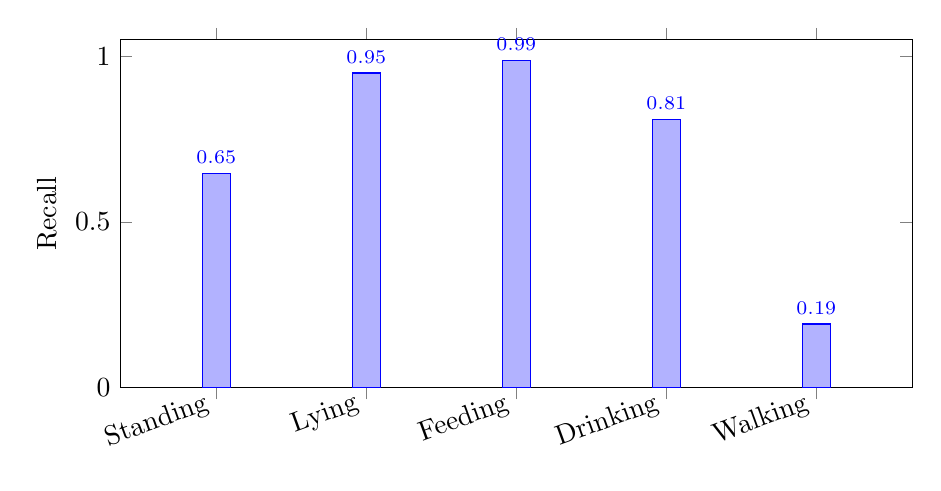
\begin{tikzpicture}
\begin{axis}[width=0.96\textwidth,height=6cm,ybar,ymin=0,ymax=1.05,
 ylabel={Recall},symbolic x coords={Standing,Lying,Feeding,Drinking,Walking},
 xtick=data,x tick label style={rotate=20,anchor=east},enlarge x limits=0.16,
 nodes near coords,point meta=y,nodes near coords style={font=\scriptsize},
 /pgf/number format/fixed,/pgf/number format/precision=2]
\addplot coordinates {(Standing,0.6460) (Lying,0.9496) (Feeding,0.9885) (Drinking,0.8095) (Walking,0.1923)};
\end{axis}
\end{tikzpicture}
\caption[Behavior test recall by class]{Recorded Behavior test recall. Walking has 26 test observations and occurs only in CVB. This reproduces recorded metrics; full-run cache verification remains open.\evidence{E09,E12}}
\label{fig:behaviorrecall}
\end{figure}


The perception pipeline retained 780 sequences (approximately 96.4\% coverage), excluding 29 sequences due to pen stanchion occlusions. Re-evaluating Run~2 on this matched cohort establishes a fair baseline for the Perception-Enhanced Temporal model (Run~5).

\begin{table}[htbp]
\centering\small
\caption[Behavior RGB and cattle-centered temporal comparison]{Behavior results. Direct comparison uses the same 780 retained test sequences; the 809-sample Run 2 row is the canonical full-test reference.\evidence{E09,E27}}
\label{tab:behaviorcomparison}
\begin{tabular}{lrrrrr}
\toprule
Configuration & $N$ & Accuracy & Bal. acc. & Macro-F1 & Loss \\
\midrule
Run 2 RGB, full test & 809 & 88.88\% & 71.72\% & 0.7413 & 0.5312 \\
Run 2 RGB, matched & 780 & \textbf{88.46\%} & 71.30\% & 0.7378 & 0.5505 \\
Run 5 perception + Conv1D & 780 & 87.44\% & \textbf{74.43\%} & \textbf{0.7397} & \textbf{0.4430} \\
\bottomrule
\end{tabular}
\end{table}


As per Table~\ref{tab:behaviorcomparison}, temporal foreground modeling has helped enhance balanced accuracy and test loss. While balanced accuracy went up from 71.30\% to 74.43\%, test loss has gone down from 0.5505 to 0.4430. However, overall accuracy was affected adversely and went down from 88.46\% to 87.44\%. This means that there is an improvement of the model for some classes but not necessarily in all measures.\evidence{E27}

\begin{table}[htbp]
\centering\small
\caption[Matched Behavior class-wise comparison]{Class-wise F1 on the matched 780-sequence Behavior test. Walking occurs only in CVB.\evidence{E27}}
\label{tab:behaviorclasscomparison}
\begin{tabular}{lrrr}
\toprule
Class & Run 2 RGB & Run 5 perception + Conv1D & Change \\
\midrule
Standing & 0.7556 & 0.7215 & $-0.0341$ \\
Lying & 0.9512 & 0.9169 & $-0.0343$ \\
Feeding & 0.9218 & 0.9465 & $+0.0247$ \\
Drinking & 0.8430 & 0.8682 & $+0.0252$ \\
Walking & 0.2174 & 0.2456 & $+0.0282$ \\
\bottomrule
\end{tabular}
\end{table}


The class-wise results (Table~\ref{tab:behaviorclasscomparison}) clarify this trade-off: dynamic and minority categories improved—most critically lifting Walking F1 from 0.2174 to 0.2456—while dominant posture categories (Standing and Lying) experienced minor declines. The combined foreground-guided temporal configuration improved selected dynamic and minority-class outcomes, while some posture-dominated classes declined.

\begin{table}[htbp]
\centering\small
\caption[Matched Behavior source-specific comparison]{Source-specific metrics on the matched Behavior test. Both sources occur in training; these are not external-transfer results.\evidence{E27}}
\label{tab:behaviorsourcecomparison}
\begin{tabular}{llrrrr}
\toprule
Source & Configuration & $N$ & Accuracy & Bal. acc. & Macro-F1 \\
\midrule
CVB & Run 2 RGB & 422 & 84.12\% & 60.62\% & 0.6541 \\
CVB & Run 5 perception + Conv1D & 422 & 80.09\% & 61.05\% & 0.6188 \\
Beef & Run 2 RGB & 358 & 93.58\% & 90.48\% & 0.9079 \\
Beef & Run 5 perception + Conv1D & 358 & 96.09\% & 94.26\% & 0.9414 \\
\bottomrule
\end{tabular}
\end{table}


Source-disjoint evaluation demonstrates pronounced domain dependence (Table~\ref{tab:behaviorsourcecomparison}). Performance on pasture cattle clips (Kaggle Beef) advanced to 96.09\% accuracy and 0.9414 Macro-F1. Conversely, authentic barn surveillance (CVB) saw overall accuracy decline from 84.12\% to 80.09\%. Because Run~5 simultaneously integrated foreground masks and 1D temporal convolution, these shifts cannot be attributed independently to mask guidance versus sequence modeling.

\subsection{Cattle Re-Identification Results}

The open set biometric identification experiment was done by using SideView Protocol~A. The system scanned through a fixed database of 36,811 images from the parlor using barn CCTV and handheld camera images. The experiment involved 69 cows that were not among the 41 training cows.\evidence{E22,E29}

\begin{table}[htbp]
\centering\small
\caption[Barn-to-Parlor Re-ID results]{Protocol A Barn-to-Parlor retrieval on 25,260 queries, 36,811 gallery images, and 69 held-out cows.\evidence{E22,E29}}
\label{tab:reidbarn}
\begin{tabular}{lrrrr}
\toprule
Configuration & Rank-1 & Rank-5 & Rank-10 & mAP \\
\midrule
Run 3 RGB & 58.64\% & \textbf{78.19\%} & \textbf{83.72\%} & 38.32\% \\
Run 6 oracle GT-guided & \textbf{63.90\%} & 77.10\% & 82.58\% & \textbf{40.68\%} \\
Change & $+5.26$ pp & $-1.09$ pp & $-1.14$ pp & $+2.36$ pp \\
\bottomrule
\end{tabular}
\end{table}


In case of Barn-to-Parlor experiments, the Oracle Segmentation-Guided model (Run~6) enhanced the main retrieval performance in Table~\ref{tab:reidbarn}. Accuracy for Rank-1 increased from 58.64\% to 63.90\%, whereas the mAP increased from 38.32\% to 40.68\%. It indicates that the model performed better when identifying the right cow among the retrieved images. But the performance on the deeper ranks was more or less similar or even worse.

\begin{table}[htbp]
\centering\small
\caption[Snapshot-to-Parlor Re-ID results]{Protocol A Snapshot-to-Parlor retrieval on 607 queries from 63 held-out cows and a 36,811-image gallery.\evidence{E22,E29}}
\label{tab:reidsnapshot}
\begin{tabular}{lrrrr}
\toprule
Configuration & Rank-1 & Rank-5 & Rank-10 & mAP \\
\midrule
Run 3 RGB & 38.88\% & 57.17\% & 64.58\% & 27.05\% \\
Run 6 oracle GT-guided & \textbf{62.93\%} & \textbf{75.29\%} & \textbf{81.05\%} & \textbf{40.42\%} \\
Change & $+24.05$ pp & $+18.12$ pp & $+16.47$ pp & $+13.37$ pp \\
\bottomrule
\end{tabular}
\end{table}


The handheld Snapshot-to-Parlor evaluation yielded a substantially larger effect (Table~\ref{tab:reidsnapshot}). Under unconstrained mobile queries, Rank-1 accuracy rose from 38.88\% to 62.93\% (+24.05 pp), alongside an mAP rise from 27.05\% to 40.42\%. The oracle target-centered configuration produced its largest improvement under the Snapshot-to-Parlor setting, where acquisition differences were greater.

These outcomes must be interpreted strictly within an oracle evaluation context. Because Run~6 uses released ground-truth masks for cropping and channel fusion, these results do not establish that automated upstream segmentation would achieve identical gains in deployment. Furthermore, target framing and mask guidance were introduced jointly, precluding isolated attribution to either factor.

\subsection{Perception Coverage and Supporting Viewpoint Evidence}

Automated upstream filtering inherently restricts evaluation scope to samples where perception succeeds. Table~\ref{tab:coverage} summarizes retention rates across the completed evaluations.

\begin{table}[htbp]
\centering\small
\caption[Perception coverage in completed enhanced evaluations]{Coverage of the cattle-centered inputs used in Runs 4--6. SideView coverage uses released ground-truth masks and is not an automatic-perception result.\evidence{E24,E26,E27,E29}}
\label{tab:coverage}
\begin{tabularx}{\textwidth}{@{}>{\raggedright\arraybackslash}p{3.2cm}>{\raggedright\arraybackslash}p{2.8cm}>{\raggedright\arraybackslash}p{1.8cm}Y@{}}
\toprule
Evaluation & Retained / candidate & Coverage & Exclusions or boundary \\
\midrule
Run 4 BCS test & 7,549 / 8,040 & 93.89\% & 489 detector and 2 SAM failures. \\
Run 5 Behavior Train+Val & 4,271 / 4,465 & 95.65\% & 194 invalid-mask exclusions. \\
Run 5 Behavior test & 780 / 809 & 96.42\% & 29 perception exclusions. \\
Run 6 SideView Protocol A & All gallery/query images & 100\% & Paired masks supplied by the dataset. \\
\bottomrule
\end{tabularx}
\end{table}


The evaluated BCS cohort covers 93.89\% of the canonical test set, while Behavior covers 96.42\% of sequences (with 29 sequences excluded due to stanchion occlusion). SideView provides complete ground-truth mask coverage across all 80,260 images, representing an oracle benchmark rather than autonomous field availability.

An auxiliary three-class viewpoint classifier (front, side, rear) achieved 86.26\% accuracy and 0.8573 Macro-F1 on 131 held-out images, confirming task feasibility on its own domain. However, because cross-domain feature transfer to the downstream task datasets was not independently validated, viewpoint conditioning was excluded from the primary multi-task pipeline.\evidence{E31}

\section{Multi-Task Learning Results}

To evaluate joint optimization across the three cattle monitoring domains, all multi-task configurations were tested on the exact matched held-out populations established for single-task references:
\begin{itemize}
 \item \textbf{Body Condition Scoring}: $N = 7{,}549$ ScienceDB images under the burst-group-disjoint protocol (identical-passage safe, not biological cow-disjoint).
 \item \textbf{Behavior Recognition}: $N = 780$ sequence samples ($T = 8$ frames; $6{,}240$ total frames) across barn CCTV (CVB, $N = 422$) and feedlot clips (Kaggle Beef, $N = 358$), with Walking exclusive to CVB.
 \item \textbf{Cattle Re-Identification}: SideView Protocol~A across 69 unseen cattle against the $36{,}811$-image parlor gallery ($25{,}260$ barn queries and $607$ snapshot queries) with released oracle target masks.
\end{itemize}
Checkpoint selection was governed strictly by minimizing composite validation loss, with held-out test sets remaining untouched until final one-time post-training evaluation.

\subsection{Body Condition Scoring Multi-Task Outcomes}

The Table~\ref{tab:mtl_bcs_results} demonstrates that BCS performance deteriorated when hard-shared multi-task approach (E1) was applied relative to the performance of the baseline (Run~4). Physical mean absolute error became equal to 0.1709 for Run~4 and 0.1788 for E1. Other metrics like tolerance accuracy and balanced performance metric became worse as well. Ordinal cross-entropy loss became somewhat better but did not contribute to the improvement of BCS score prediction.

\begin{table}[htbp]
\centering\small
\caption[Multi-task Body Condition Scoring results]{Multi-task Body Condition Scoring results on the matched held-out ScienceDB test population ($N = 7{,}549$ images). For MAE and Loss, lower values are better ($\downarrow$); for Acc@1, Acc@0, Balanced Accuracy, and Macro-F1, higher values are better ($\uparrow$). All models share the four-channel ResNet-18 spatial trunk.\evidence{E24,E36,E37,E38}}
\label{tab:mtl_bcs_results}
\setlength{\tabcolsep}{2pt}
\begin{tabular}{lrrrrrr}
\toprule
\textbf{Configuration} & \textbf{MAE} & \textbf{Acc@1} & \textbf{Acc@0} & \textbf{Bal.~Acc.} & \textbf{Macro-F1} & \textbf{Loss} \\
\midrule
Single-Task Reference (Run 4) & \textbf{0.1709} & \textbf{89.40\%} & \textbf{43.57\%} & \textbf{39.70\%} & \textbf{0.4039} & 0.4403 \\
Monolithic Hard-Shared (E1) & 0.1788 & 88.44\% & 41.10\% & 35.70\% & 0.3605 & \textbf{0.4175} \\
Modular Task-Private (E3) & 0.1916 & 86.32\% & 38.47\% & 33.13\% & 0.3291 & 0.4555 \\
PCGrad Hard-Shared (E4) & 0.1828 & 87.84\% & 40.23\% & 34.97\% & 0.3516 & 0.4181 \\
\bottomrule
\end{tabular}
\end{table}


Neither modular adapters nor gradient projection overcame this performance deficit. Introducing task-private bottleneck adapters (E3) degraded performance further, resulting in the highest error across all models ($\mathrm{MAE} = 0.1916$). The PCGrad Hard-Shared Optimization Control (E4) partially mitigated this loss, lowering MAE to 0.1828 and recovering tolerance accuracy relative to E3. However, E4 still trailed the dedicated single-task reference ($\mathrm{MAE} = 0.1709$). Crucially, all three multi-task configurations underperformed the single-task model on primary physical and balanced metrics, confirming persistent negative transfer for body condition scoring under joint training.

\subsection{Behavior Recognition Multi-Task Outcomes}

Joint training under naive hard sharing (E1) produced severe degradation across balanced evaluation measures (Table~\ref{tab:mtl_behavior_results}). Balanced accuracy plunged from 74.43\% in the single-task reference to 67.30\%, accompanied by sharp declines in overall accuracy and Macro-F1. The minority Walking class was disproportionately impacted, decreasing from an F1 of 0.2456 to 0.0408. Modular adapters (E3) offered only selective, loss-specific relief; while E3 improved test loss and overall accuracy, balanced accuracy eroded further (66.70\%) and Walking F1 fell to 0.0000.

\begin{table}[htbp]
\centering\small
\caption[Multi-task Behavior Recognition results]{Multi-task Behavior Recognition results on the matched held-out test population ($N = 780$ sequences, $T = 8$ frames). Higher values are better ($\uparrow$) for accuracy and F1 metrics; lower values are better ($\downarrow$) for loss. The single-task reference is Run 5.\evidence{E27,E33}}
\label{tab:mtl_behavior_results}
\setlength{\tabcolsep}{2.2pt}
\begin{tabular}{lrrrrr}
\toprule
\textbf{Configuration} & \textbf{Accuracy} & \textbf{Bal.~Acc.} & \textbf{Macro-F1} & \textbf{Loss} & \textbf{Walking F1} \\
\midrule
Single-Task Reference (Run 5) & \textbf{87.44\%} & \textbf{74.43\%} & \textbf{0.7397} & 0.4430 & \textbf{0.2456} \\
Monolithic Hard-Shared (E1) & 85.00\% & 67.30\% & 0.6866 & 0.6226 & 0.0408 \\
Modular Task-Private (E3) & 85.77\% & 66.70\% & 0.6755 & \textbf{0.4193} & 0.0000 \\
PCGrad Hard-Shared (E4) & 86.92\% & 69.15\% & 0.7114 & 0.5454 & 0.0909 \\
\bottomrule
\end{tabular}
\end{table}


The PCGrad optimization control (E4) was the most effective multi-task variant for Behavior, partially mitigating hard-sharing degradation. E4 raised balanced accuracy to 69.15\% and recovered Walking F1 to 0.0909 (more than doubling E1). Moreover, on authentic CVB barn surveillance (Table~\ref{tab:mtl_behavior_source}), E4 reached an overall accuracy of 81.04\%, marginally surpassing the single-task reference. However, source-disjoint results emphasize that overall accuracy and class-balanced fidelity diverge: CVB balanced accuracy (55.30\%) and Walking F1 under E4 remained far below the dedicated single-task reference (61.05\% and 0.2456, respectively). Thus, while PCGrad provided clear optimization-level mitigation, it did not fully restore single-task discriminative power on difficult minority states.

\begin{table}[htbp]
\centering\footnotesize
\caption[Multi-task Behavior source-disjoint breakdown]{Multi-task Behavior Recognition performance breakdown across acquisition sources: authentic barn surveillance (CVB, $N = 422$) and feedlot camera clips (Kaggle Beef, $N = 358$). Note that the minority Walking class is exclusive to CVB.\evidence{E27,E33}}
\label{tab:mtl_behavior_source}
\setlength{\tabcolsep}{1.4pt}
\begin{tabular}{lrrrrrr}
\toprule
& \multicolumn{3}{c}{\textbf{CVB Barn CCTV ($N = 422$)}} & \multicolumn{3}{c}{\textbf{Kaggle Beef Feedlot ($N = 358$)}} \\
\cmidrule(lr){2-4} \cmidrule(lr){5-7}
\textbf{Configuration} & \textbf{Accuracy} & \textbf{Bal.~Acc.} & \textbf{Macro-F1} & \textbf{Accuracy} & \textbf{Bal.~Acc.} & \textbf{Macro-F1} \\
\midrule
Single-Task (Run 5) & 80.09\% & \textbf{61.05\%} & \textbf{0.6188} & \textbf{96.09\%} & \textbf{94.26\%} & \textbf{0.9414} \\
Hard-Shared Control (E1) & 76.78\% & 48.90\% & 0.5402 & 94.69\% & 93.11\% & 0.9236 \\
Modular Task-Private (E3) & 80.33\% & 60.61\% & 0.6026 & 92.18\% & 87.29\% & 0.8849 \\
PCGrad Hard-Shared (E4) & \textbf{81.04\%} & 55.30\% & 0.6141 & 93.85\% & 92.05\% & 0.9158 \\
\bottomrule
\end{tabular}
\end{table}


\subsection{Cattle Re-Identification Multi-Task Outcomes}

The dedicated single-task oracle model (Run~6) maintained the strongest performance across both query settings, achieving a Rank-1 accuracy of 63.90\% on Barn queries and 62.93\% on Snapshot queries, with mAP exceeding 40\% in both environments (Table~\ref{tab:mtl_reid_results}). Monolithic hard sharing (E1) degraded these principal retrieval measures considerably, dropping Barn Rank-1 to 57.38\% and Snapshot Rank-1 to 57.17\%, alongside substantial losses in ranking precision ($\mathrm{mAP}$).

\begin{table}[htbp]
\centering\small
\caption[Multi-task Cattle Re-Identification results under SideView Protocol A]{Multi-task Cattle Re-Identification retrieval under SideView Protocol A on 69 unseen cattle identities evaluated against the 36,811-image fixed parlor gallery. Evaluated with released SideView target masks matching the oracle single-task reference (Run 6).\evidence{E29,E34}}
\label{tab:mtl_reid_results}
\begin{tabular}{lrrrr}
\toprule
\textbf{Configuration / Model} & \textbf{Rank-1} $\uparrow$ & \textbf{Rank-5} $\uparrow$ & \textbf{Rank-10} $\uparrow$ & \textbf{mAP} $\uparrow$ \\
\midrule
\multicolumn{5}{l}{\textit{Barn-to-Parlor Video Queries ($25{,}260$ queries)}} \\
\midrule
Single-Task Reference (Run 6) & \textbf{63.90\%} & \textbf{77.10\%} & \textbf{82.58\%} & \textbf{40.68\%} \\
Monolithic Hard-Shared (E1) & 57.38\% & 73.33\% & 79.79\% & 30.37\% \\
Modular Task-Private (E3) & 49.08\% & 67.72\% & 75.03\% & 28.04\% \\
PCGrad Hard-Shared (E4) & 54.97\% & 68.81\% & 74.99\% & 30.23\% \\
\midrule
\multicolumn{5}{l}{\textit{Snapshots-to-Parlor Handheld Queries ($607$ queries)}} \\
\midrule
Single-Task Reference (Run 6) & \textbf{62.93\%} & 75.29\% & 81.05\% & \textbf{40.42\%} \\
Monolithic Hard-Shared (E1) & 57.17\% & \textbf{75.45\%} & \textbf{82.70\%} & 33.69\% \\
Modular Task-Private (E3) & 53.71\% & 72.32\% & 80.23\% & 28.78\% \\
PCGrad Hard-Shared (E4) & 57.00\% & 72.16\% & 78.25\% & 33.87\% \\
\bottomrule
\end{tabular}
\end{table}


Different results were obtained from the architecture and optimization approaches in Re-ID. The modular adapters (E3) approach decreased the performance to Barn Rank-1 of 49.08\%. PCGrad (E4) improved the performance in comparison with the previous one, and achieved a result of Barn Rank-1 of 54.97\%, and a higher value of Snapshot mAP of 33.87\%. Nevertheless, its results were inconsistent with E1 and were still lower than those of the single-task network. Minor improvements occurred at higher ranks, for example, Snapshot Rank-10 was slightly increased in E3. It can be concluded that there is a difference in the retrieval performance by the implementation of multiple tasks for feature sharing; however, this method is still not as accurate as a specific single-task Re-ID approach.

\subsection{Observed Shared-Backbone Gradient Conflict}

Table~\ref{tab:pcgrad_diagnostics} reports the gradient conflict diagnostics recorded during E4 PCGrad training across all 30 epochs ($16{,}140$ super-steps). Across this schedule, the diagnostics engine recorded 44,177 pairwise conflict projections, averaging 2.737 projections per super-step (out of a theoretical maximum of 6). Conflict frequencies were remarkably uniform across task pairings: BCS and Behavior gradients conflicted in 47.8\% of super-steps, BCS and Re-ID in 46.5\%, and Behavior and Re-ID in 47.4\%.

\begin{table}[htbp]
\centering\small
\caption[PCGrad shared-backbone gradient conflict diagnostics]{Observed shared-backbone gradient conflict diagnostics recorded during E4 PCGrad multi-task training across all 30 epochs ($16{,}140$ super-steps). Conflicts were evaluated pairwise on the shared four-channel ResNet-18 parameter gradients prior to projection surgery.\evidence{E35}}
\label{tab:pcgrad_diagnostics}
\begin{tabularx}{\textwidth}{Xr}
\toprule
\textbf{Diagnostic Metric / Evaluated Task Pair} & \textbf{Observed Training Quantity} \\
\midrule
BCS vs. Behavior Gradient Conflict Frequency & 47.8\% of super-steps \\
BCS vs. Re-ID Gradient Conflict Frequency & 46.5\% of super-steps \\
Behavior vs. Re-ID Gradient Conflict Frequency & 47.4\% of super-steps \\
\midrule
Total Executed Multi-Task Super-Steps & 16,140 \\
Total Triggered Pairwise Conflict Projections & 44,177 \\
Mean Conflict Projections per Super-Step (out of 6 max) & 2.737 \\
\bottomrule
\end{tabularx}
\end{table}


As per the training diagnostics, conflicting gradients are observed quite often in the four-channel ResNet-18 backbone that is shared by both tasks. Nevertheless, one has to make sure that an essential distinction between E1 and E4 is not forgotten. E1 just summed up the gradients, whereas E4 applied the PCGrad method in order to determine the conflicting gradient directions and to project them. As a result, the E4 results demonstrate that conflicts are often observed only in the case of E4 training. They cannot be used in arguing that E1 experienced an equivalent rate of conflict or that gradient interference is the only explanation for the performance difference.

\section{Analysis of Multi-Task Design Solutions}

The empirical evaluations across single-task and multi-task configurations support distinct findings regarding the three multi-task design hypotheses:
\begin{enumerate}
 \item \textbf{Monolithic Hard Parameter Sharing (E1)}: In the case of the Monolithic Hard Parameter Sharing model (E1), all three tasks used a single shared ResNet-18 spatial backbone. In doing so, worse results were obtained for BCS, Behavior, and Re-ID. These findings indicate the presence of negative transfer and that the three tasks do not necessarily have to reinforce each other. The three tasks differ in the type of information used; body shape is used in BCS, motion in Behavior, and subtle visual cues in Re-ID. However, E1 does not allow us to specify precisely what was affected. E1 is unable to provide exact information about the impact on the common characteristics.
 \item \textbf{Modular Task-Private Adapters (E3)}: The Modular Task-Private Adapters (E3) introduced separate adapter blocks for each task between the backbone and the prediction head, yet the problem of negative transfer was not solved consistently. While some surveillance and loss measures have become better, BCS and Re-ID measures worsened, as well as Behavior balance accuracy. In addition to this, 395,904 trainable parameters were added in E3, making an increase of model capacity by 3.32\%. This is why the improvements of the performance cannot be explained solely by task-specific routing.
 \item \textbf{PCGrad Optimization Control (E4)}: Model (E4) PCGrad modified the optimization process without modifying the model size. The number of trainable parameters in E4 was the same as that of E1, which is 11,926,706, while there were no adapter layers in it. PCGrad could address the negative transfer problem in some aspects, like Behavior accuracy, balanced accuracy, Macro-F1, and CVB surveillance effectiveness. PCGrad did better in important results of BCS and Re-ID than E3. Nevertheless, E4 was worse than single-task models on some major criteria.
\end{enumerate}

Table~\ref{tab:decisions} synthesizes the key design decisions and empirical dispositions established across the single-task and multi-task investigations.

\begin{table}[htbp]
\centering\small
\caption[Evidence-led design decisions]{Design decisions established before the final MTL experiments.\evidence{E01,E04,E06,E11,E13,E24,E27,E29,E31}}\label{tab:decisions}
\begin{tabularx}{\textwidth}{lYY}
\toprule
Question & Evidence & Disposition \\
\midrule
ScienceDB grouping & Identity semantics and overlap audit & Repaired burst groups. \\
Behavior source & Dense-video/provenance audit & CVB + Beef; MmCows external. \\
Re-ID source & MultiCam access blocker & Approved SideView contingency. \\
BCS representation & Matched Run 1/4 comparison & RT-DETR crop + binary SAM mask channel retained. \\
Behavior representation & Matched Run 2/5 comparison & Eight-frame RGB+mask + lightweight Conv1D retained. \\
Re-ID representation & Protocol A Run 3/6 comparison & Oracle GT crop+mask used as upper-bound condition. \\
Pose & Unreliable reviewed rear views & Excluded from Runs 4--6. \\
Viewpoint & Separate held-out result; transfer unverified & Not fused into Runs 4--6. \\
MTL sharing & Runs 7/8 not executed & Hard sharing vs modular design remains pending. \\
\bottomrule
\end{tabularx}
\end{table}


These outcomes demonstrate that neither simple modular adapters nor gradient projection fully mitigated negative transfer across all evaluated cattle monitoring tasks. Dedicated single-task representations remained superior on several task-specific measures, reinforcing the thesis conclusion that representation requirements are task-dependent and that multi-task integration involves metric-dependent trade-offs.

\section{Statistical Analysis and Uncertainty Boundaries}

All single-task baselines and multi-task configurations in this chapter are evaluated as single trained checkpoints (point estimates). Repeated-seed training distributions, confidence intervals, and hypothesis tests were not computed. Consequently, reported differences are descriptive point comparisons and are not characterized as statistically significant.

The matched-sample design ensures valid internal comparisons across identical test cohorts: 7,549 ScienceDB images for BCS, 780 sequences for Behavior, and SideView Protocol~A for Re-ID. However, this control does not quantify seed variability or population variance, and correlated video frames or bursts must not be treated as independent biological samples.

Similarly, recorded PCGrad conflict frequencies (Table~\ref{tab:pcgrad_diagnostics}) represent descriptive training diagnostics from a single optimization trajectory. Marginal metric differences (such as E4 vs. E1 on snapshot mAP of $+0.18$ pp) cannot be claimed as statistically equivalent.

\section{Cross-Task Relationships and Claim Boundaries}

The three evaluation domains employ incommensurable metrics with distinct scales and optimization objectives:
\begin{itemize}
 \item BCS uses physical Mean Absolute Error in BCS units (lower is better), Acc@1 within $\pm 0.25$ units, and exact ordinal accuracy.
 \item Behavior uses overall accuracy, balanced accuracy, Macro-F1 across five classes, and per-class F1-scores (higher is better).
 \item Re-ID uses cumulative match characteristics (Rank-1, Rank-5, Rank-10) and mean Average Precision across open-set rankings (higher is better).
\end{itemize}
Because these metrics cannot be meaningfully combined into an aggregate score, negative transfer must be evaluated within each domain against its matched single-task reference.

The evaluation cohorts also define strict generalization boundaries:
\begin{itemize}
 \item ScienceDB evaluates unseen burst groups from automated passage sequences, not verified unseen biological cows.
 \item Behavior evaluates protected video recordings and sessions, not cow-disjoint herds; Walking is evaluated solely within CVB barn surveillance.
 \item SideView Protocol~A: The test comprises 69 biologically unique cows which have been left out of the representation learning process. However, the Re-ID systems rely on the ground-truth masks which have been released. It means that the results of the tests have been obtained using an oracle segmentation framework.
\end{itemize}
The external datasets mentioned in the bigger scheme of the research, including Ruchay, Dryad, MmCows, CBVD-5, and BECA, have not yet been validated. They are scheduled for stress testing in the future. Simply by referring to these datasets, we cannot imply that the model will generalize to other datasets/environments.

\section{Discussion of Findings}

The empirical findings presented in this chapter synthesize into three overarching insights:

In fact, applying visual information about cattle is quite useful in single task tests compared to RGB pictures. Nevertheless, the advantages of such approach may differ from task to task. Localized cropping and binary mask guidance improved physical score proximity for BCS (Table~\ref{tab:bcscomparison}) and elevated open-set retrieval under unconstrained handheld camera angles for Re-ID (Table~\ref{tab:reidsnapshot}). For Behavior, temporal foreground modeling improved class-balanced discrimination and minority-class detection while redistributing accuracy across sources (Tables~\ref{tab:behaviorcomparison}--\ref{tab:behaviorsourcecomparison}). These gains demonstrate the value of isolating animal foregrounds, while underscoring that foreground guidance does not operate as an unconditional panacea across all sub-metrics.

Second, monolithic hard parameter sharing produced consistent outcome-level negative transfer across all three domains. Relative to matched single-task baselines, joint training under a single shared backbone degraded BCS physical error (Table~\ref{tab:mtl_bcs_results}), depressed Behavior balanced accuracy and minority walking recognition (Table~\ref{tab:mtl_behavior_results}), and diminished primary Re-ID retrieval precision (Table~\ref{tab:mtl_reid_results}). These matched degradations do not support an assumption of automatic benefit from hard sharing across these heterogeneous tasks.

Third, neither architectural capacity expansion nor gradient projection universally resolved this cross-task interference. Adding task-private residual bottleneck adapters (E3) yielded selective loss improvements for behavior surveillance but exacerbated degradations in body condition scoring and biometric retrieval. Optimization-level gradient projection (E4) provided more effective, selective mitigation—achieving the strongest multi-task behavior metrics and recovering ground on ordinal scoring and retrieval under exact parameter parity with the hard-shared baseline. Empirical training diagnostics (Table~\ref{tab:pcgrad_diagnostics}) confirm that opposing shared-backbone gradients occurred frequently throughout joint optimization.

Nevertheless, dedicated single-task models preserved superior performance across the principal benchmarks of all three domains. Rather than demonstrating universal synergy from joint learning, the findings are consistent with task-dependent representation and optimization requirements that are not fully served by a single shared backbone. Multi-task agricultural monitoring therefore demands careful metric-aware trade-off analysis rather than naive joint consolidation.
